\documentclass{article}
\usepackage{microtype}\usepackage{graphicx}\usepackage{booktabs}\usepackage{hyperref}\usepackage{amsmath}\usepackage{amssymb}\usepackage{longtable}\usepackage{array}\usepackage{calc}
\newcommand{\tightlist}{\setlength{\itemsep}{0pt}\setlength{\parskip}{0pt}}
\providecommand{\real}[1]{#1}
\usepackage{icml2025}
\icmltitlerunning{Three Numbers per Rater}
\begin{document}
\twocolumn[
\icmltitle{Three Numbers per Rater: Disagreement in Preference Data Is How People Use the Scale}
\begin{icmlauthorlist}\icmlauthor{Anonymous Authors}{anon}\end{icmlauthorlist}
\icmlaffiliation{anon}{Anonymous Institution}
\icmlcorrespondingauthor{Anonymous}{anon@example.com}
\vskip 0.3in]
\printAffiliationsAndNotice{}
\begin{abstract}
Pluralistic alignment trains reward models that represent disagreement among people --- as a distribution over ratings, as demographic groups, or as a learned user latent. All three assume that what makes people disagree is something a model should learn from the text or from who the people are. We measure, on three public multi-rater datasets (MultiPref pairwise preferences, DICES conversational-safety ratings, PRISM response ratings), where the reproducible structure of disagreement actually sits. Split-half analysis shows that the shape of the rating distribution beyond its location is poorly reproducible across rater panels (split-half reliability 0.25 on MultiPref), that about a tenth of the reproducible part is decodable from a frozen LLM representation of the text, and that rater-side structure dominates item-side dispersion by a factor of 25 in held-out likelihood. Acting on this, we model each rater by a few text-independent offsets on the reward model's output --- how they use the scale --- learned from a handful of their ratings. For raters never seen in training, offsets fitted on 20 ratings improve held-out log-likelihood over a distributional reward model by 0.08--0.10 nats per rating on all three datasets, while demographic or crowd/expert groups improve it by at most 0.003, a tuned 8-dimensional text-interacting user latent does no better, and reimplementations of two published personalised reward models (VPL, PAL) gain less; on binary preference labels none of the methods personalises at all. On pairwise preferences, a symmetric three-parameter version (how often a rater says ``clearly'', ``slightly'', ``tie'') is the best model at every number of shots and also improves predicting which response the rater prefers; adding an A-vs-B position term from few ratings hurts. What the offsets encode is task-specific: rating intensity on two-sided preference scales, leniency on single-response ratings. On top of a LoRA-fine-tuned reward model the gain is unchanged (+0.100) and adds to the fine-tuning gain, and it exceeds what the same LLM learns from the rater's ratings placed in its prompt (+0.042).
\end{abstract}
\section{Introduction}

Reward models and LLM judges are trained on human ratings that disagree. A recent line of work treats this disagreement as signal to be modelled rather than noise to be averaged: distributional preference learning estimates a distribution over each alternative's utility rather than a point score (\citealp{siththaranjan2024dpl}); jury learning predicts individual annotators from content, annotator and demographic-group embeddings (\citealp{gordon2022jury}), and large datasets such as PRISM are analysed by sociodemographic group (\citealp{kirk2024prism}); personalised reward models learn a per-user latent, inferred for a new user from a few examples (\citealp{poddar2024vpl}; \citealp{chen2025pal}). The pluralistic-alignment agenda (\citealp{sorensen2024roadmap}) makes the representation of disagreement a first-class goal.

These approaches agree on one premise: the disagreement worth modelling is a property of the \emph{item} (some responses are contested) or of \emph{who the raters are} (groups and individuals hold different values about content). There is a third, older possibility that measurement theory takes for granted and reward modelling largely does not: raters differ in \textbf{how they use the response scale} --- some say ``clearly better'' where others say ``slightly better'', some rarely call a tie, some are harsher across the board (\citealp{linacre1989mfrm}; \citealp{baumgartner2001response}). Such response styles are text-independent, cheap to estimate, and invisible to a model that only conditions on content or demographics.

We ask two questions. \textbf{(Q1, measurement)} In public multi-rater preference and rating data, how much of the disagreement is reproducible across raters, how much of the reproducible part is in the text, and how much is rater-side? \textbf{(Q2, modelling)} If the answer is ``mostly rater-side'', what is the cheapest rater model that captures it for a \emph{new} rater from few ratings --- and how does it compare with distributional, group-conditioned and low-rank personalised reward models under the same protocol?

\textbf{Contributions.} (1) A learner-free measurement of disagreement in preference data --- split-half reliability of the distribution's shape, cross-fitted text decodability, and a rater--item decomposition of held-out likelihood --- showing that rater-side structure dominates (\S{}3). (2) A factorised reward model: a text model for the item, and a few text-independent offsets per rater on its output, shrunk toward the population and adapted from k ratings (\S{}4). (3) A new-rater, few-shot evaluation on three datasets against distributional, group-conditioned and low-rank-latent reward models, with all hypotheses, amendments and failures pre-registered and reported (\S{}5): offsets beat groups everywhere, match a tuned low-rank latent, and a symmetric three-number style model is best on pairwise preferences. (4) The observation that what ``style'' means depends on the scale: intensity on two-sided preferences, leniency on single-response ratings (\S{}5.3).

\section{Related work}

\textbf{Pluralistic and distributional reward models.} Distributional preference learning (\citealp{siththaranjan2024dpl}), diverging-preference detection (\citealp{zhang2025diverging}), PRISM (\citealp{kirk2024prism}), MultiPref (\citealp{miranda2025hybrid}) and DICES (\citealp{aroyo2023dices}) motivate modelling disagreement; jury learning (\citealp{gordon2022jury}) and multi-annotator models (\citealp{davani2022dealing}) predict individual annotators. \textbf{Personalised reward models} infer a user latent from a few examples (\citealp{poddar2024vpl}; \citealp{chen2025pal}) or learn per-user embeddings jointly with the reward model (\citealp{li2024prlhf}). \textbf{Annotator demographics} as predictors of labels have been found weak in several studies (e.g.~\citealp{orlikowski2023ecological}). \textbf{Measurement theory}: rater severity and scale use are standard facets in many-facet Rasch measurement (\citealp{linacre1989mfrm}; \citealp{eckes2011mfrm}) and response styles are a classical survey-methods topic (\citealp{baumgartner2001response}). We connect the last line to the first: for new-rater prediction, the measurement-theory rater facet is what the reward model is missing.

\section{Where does disagreement in preference data sit? (Q1)}

\textbf{Data.} MultiPref (\citealp{miranda2025hybrid}; 10,461 comparisons; 4 ratings each by 2 crowd and 2 expert raters; 227 persistent raters; 5 ordered levels A-clearly \ldots{} B-clearly). PRISM (\citealp{kirk2024prism}; 68,371 responses each rated 1--100 by one of 1,396 users; binned to 5 fixed levels). DICES-350 (\citealp{aroyo2023dices}; 350 conversations fully crossed with 104 quality-checked raters; safe / unsure / unsafe).

\textbf{Estimators.} For an item with ratings on \(K\) ordered levels, let \(h\) be the empirical rating distribution and \(C\) the cumulative operator. Split the item's raters at random into disjoint panels \(P_1\) (\(a\) raters) and \(P_2\), and let \(q\) be a cross-fitted \emph{location-only} forecast with exactly the mode and mean of \(P_1\) (built from other items in the same mode-and-mean cell). With \(r_1 = C(h_1 - q)\), \(r_2 = C(h_2 - q)\), \(M = \|r_1\|^2/n\) and \(X = \langle r_1, r_2\rangle/n\), the forecasting value of the raw distribution over its own location obeys the identity \(S(h_1) - S(q) = M - 2X\) under the ranked probability score, so \(\rho = X/M\) is a split-half reliability of the distribution's \emph{shape} and the raw distribution beats its location exactly when \(\rho > 1/2\). Text decodability is the proper-score gain \(G = (2\langle \hat r, r_2\rangle - \|\hat r\|^2)/n\) of a residual \(\hat r\) decoded from frozen text features, cross-fitted over prompt groups, reported as the fraction \(G/X\) of the reproducible shape. The rater--item decomposition fits ordered-probit models \(Y^*_{ir} = \theta_i + \delta_r + \sigma_i\sigma_r\varepsilon\) with item locations \(\theta_i\), rater shifts \(\delta_r\), rater scales \(\sigma_r\) and item dispersions \(\sigma_i\), compares held-out likelihood over random cells (every held-out rater and item appears in training), and chooses all penalties by inner cross-validation.

\textbf{Reproducibility.} With the split-half estimator of a companion study (anonymised), the reliability of the rating distribution's shape beyond its exact mode and mean is $\rho$ = 0.25 {[}0.22, 0.29{]} on MultiPref overall preference with three raters (helpful 0.29, harmless 0.21): the raw few-rater distribution forecasts a new rater worse than its own location ($\rho$ \textless{} $\tfrac12$). \textbf{Text decodability.} A cross-fitted ridge decoder on frozen Qwen2.5-7B-Instruct features, scored on an independent rater panel, recovers G/X = 10.5 \% {[}5.7 \%, 11.9 \%{]} of the reproducible shape (within-cell permutation control $\leq$ 0; positive control 0.35) --- more than on ordinal quality ratings ($\leq$ a few percent) and less than on NLI (17--26 \%). \textbf{Rater vs item.} A long-format ordered-probit decomposition with real rater identities and penalties tuned by inner cross-validation: rater-specific thresholds improve held-out likelihood by +0.036 nats per rating over item location alone, item-specific dispersion by a further +0.0014 (ratio 25); of the rater part, rater scale contributes +0.031 and rater shift +0.005.

The reproducible part of preference disagreement is therefore mostly rater-side, and mostly about scale use.

\section{A factorised reward model (Q2)}

Let $\ell$(x) $\in$ R\^{}K be the class logits of a text-only distributional reward model for item x (K ordered rating levels). For rater r we add a text-independent offset vector: p(y \textbar{} x, r) = softmax($\ell$(x) + b\_r). Variants: \textbf{DF} (b\_r $\in$ R\^{}K, free), \textbf{DFs} (two-sided preference scales only: b\_r tied symmetrically, (e, s, t, s, e) --- extreme, slight, tie --- 3 parameters, no A-vs-B position term). Rater offsets have a Gaussian prior centred on the training-rater mean; a new rater's offsets are the MAP estimate from k of their ratings with the text model frozen. Baselines under the same protocol: \textbf{D} (text-only distributional RM), \textbf{DG} (group offsets: crowd/expert, race, region), \textbf{DL} (low-rank text-interacting latent: $\ell$(x) + (Wx + w$_0$)$\cdot$z\_r, d = 8, the personalised-RM family). An interpretable probit family (rater shift / log-scale on an ordered-probit text head) is reported as a secondary analysis.

\textbf{Training and adaptation.} The text model and the training raters' offsets are fitted jointly by penalised maximum likelihood, \[\min \sum_{(i,r,y)} -\log p(y \mid x_i, r) + \lambda_{\text{text}} \|V\|^2 + \lambda_r \sum_r \|b_r\|^2,\] with \(\lambda_{\text{text}}\) chosen on the text-only model and \(\lambda_r\) on held-out items of the training raters. A new rater \(r^*\) is adapted from \(k\) ratings \(\{(x_j, y_j)\}\) by \(\hat b_{r^*} = \arg\min_b \sum_j -\log \mathrm{softmax}(\ell(x_j) + b)_{y_j} + \lambda_r \|b - \bar b\|^2\), with \(\bar b\) the training-rater mean (the prior mean; \(\hat b = \bar b\) at \(k = 0\)) and the text model frozen --- a convex problem in 3--5 parameters, solved in milliseconds. Any text model that outputs graded log-probabilities can be used: we use a ridge head on frozen LLM features (\S{}5.1--5.3), a LoRA-fine-tuned LLM reward model (\S{}5.4) and the decoder of a published personalised reward model (\S{}5.5).

\section{Experiments}
\begin{figure*}[t]\centering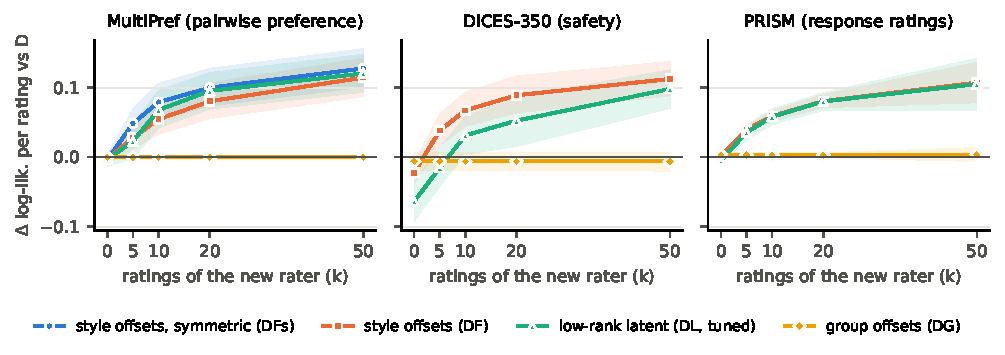
\includegraphics[width=\textwidth]{fig_main.pdf}
\caption{New raters: gain in held-out log-likelihood per rating over the text-only distributional reward model (D), as a function of the number k of the new rater's ratings used for adaptation; 95\% rater-cluster bootstrap bands, 5 folds. Text-independent rater offsets (DF; symmetric three-parameter DFs on two-sided preferences) gain 0.08--0.10 nats per rating at k = 20 on all three datasets; group offsets (crowd/expert, race, region) gain nothing; a low-rank text-interacting rater latent with a few-shot-tuned prior is at best equal.}\label{fig:main}\end{figure*}

\textbf{Protocol.} 5 folds; in each, 20 \% of raters (stratified by group) and 20 \% of prompt groups are held out; models are trained on training raters $\times$ training items with penalties chosen on a validation split; each test rater is adapted on k $\in$ \{0, 5, 10, 20, 50\} of their ratings of \emph{training} items (5 random draws) and evaluated on their ratings of \emph{held-out} items. Primary metric: held-out log-likelihood per rating; also RPS and preference-direction accuracy; rater-cluster bootstrap (B = 2,000). Text model in \S{}5.1--5.3: frozen Qwen2.5-7B features with a ridge head; \S{}5.4: a LoRA-fine-tuned reward model.

\subsection{Main result (MultiPref)}

Figure 1 shows the gain over the text-only reward model as a function of k on all three datasets. \textbar{} k \textbar{} DF $-$ D \textbar{} DFs $-$ D \textbar{} DG $-$ D \textbar{} DL $-$ D (tuned prior) \textbar{} DFs $-$ DL (tuned) \textbar{} \textbar---\textbar---\textbar---\textbar---\textbar---\textbar---\textbar{} \textbar{} 5 \textbar{} +0.028 {[}+0.012, +0.044{]} \textbar{} +0.048 {[}+0.029, +0.070{]} \textbar{} $\approx$ 0 \textbar{} +0.023 {[}$-$0.002, +0.047{]} \textbar{} +0.026 {[}+0.016, +0.037{]} \textbar{} \textbar{} 20 \textbar{} +0.080 {[}+0.055, +0.106{]} \textbar{} \textbf{+0.100 {[}+0.074, +0.128{]}} \textbar{} $\approx$ 0 \textbar{} +0.095 {[}+0.069, +0.122{]} \textbar{} +0.0045 {[}$-$0.0004, +0.0092{]} \textbar{} \textbar{} 50 \textbar{} +0.114 {[}+0.087, +0.142{]} \textbar{} +0.128 {[}+0.101, +0.156{]} \textbar{} $\approx$ 0 \textbar{} +0.120 \textbar{} +0.007 {[}+0.002, +0.013{]} \textbar{} Preference-direction accuracy (D: 0.674): DFs +0.005 {[}+0.001, +0.008{]} at k = 20; DF $-$0.014 {[}$-$0.020, $-$0.007{]}. A three-number style model gains as much as a tuned 8-dimensional text-interacting latent and more at k $\leq$ 10; fitting a rater's A-vs-B position from few ratings costs direction accuracy.

\subsection{Replications (k = 20)}

{\def\LTcaptype{none} % do not increment counter
\begin{table*}[t]\centering\footnotesize\begin{tabular}{@{}
  l
  l
  l
  l
  l@{}}
\toprule\noalign{}
dataset & DF $-$ D & DG $-$ D (groups) & DF $-$ DL (tuned prior) & direction acc. DF $-$ D \\
\midrule\noalign{}

\bottomrule\noalign{}

DICES-350 (safety) & +0.089 {[}+0.064, +0.117{]} & $-$0.006 (race) & +0.037 {[}+0.022, +0.053{]} & +0.048 {[}+0.025, +0.076{]} \\
PRISM (ratings) & +0.080 {[}+0.071, +0.090{]} & +0.003 (region) & $-$0.001 {[}$-$0.006, +0.003{]} & +0.005 {[}+0.001, +0.009{]} \\
\end{tabular}\end{table*}
}

\subsection{What the offsets encode}

In the probit family, rater \emph{scale} matters more than rater \emph{shift} on MultiPref (+0.036 {[}+0.020, +0.057{]} at k = 20), but rater \emph{shift} dominates on DICES ($-$0.053) and PRISM ($-$0.031): leniency/strictness on single-response rating scales, intensity on two-sided preference scales.

\subsection{On a fine-tuned reward model}

With a LoRA-fine-tuned Qwen2.5-7B reward model (D-LoRA, trained per fold on the training raters' rating distributions) as the text model, the three-number style model still adds +0.100 {[}+0.071, +0.130{]} nats per rating at k = 20 --- exactly its gain on the frozen-feature head. Fine-tuning improves the text-only model by +0.027 {[}+0.016, +0.039{]} (direction accuracy +1.4 points) and the style model by the same +0.027: the two gains add. Personalising the frozen-feature model with 20 ratings per rater gains more than fine-tuning the text model (+0.072 {[}+0.041, +0.106{]}). DFs keeps the direction accuracy of D-LoRA (+0.002 {[}$-$0.002, +0.006{]}). Against in-context personalisation --- the same LoRA recipe trained with ten of the rater's other ratings in the prompt and evaluated with the new rater's k ratings in the prompt (two folds, 86--90 raters) --- the three offsets on D-LoRA are better at k = 5 (+0.041 {[}+0.016, +0.065{]} nats per rating) and at k = 20 (+0.042 {[}+0.020, +0.065{]}), and more accurate on which response the rater prefers (+2.9 points); the in-context model learns from the history (+0.048 over D-LoRA) but loses 3.0 points of direction accuracy, at several thousand prompt tokens per prediction.

\subsection{Published personalised reward models}

We reimplemented VPL (\citealp{poddar2024vpl}) and PAL-B (\citealp{chen2025pal}) from their official code as heads on the same frozen per-response embeddings and evaluated them under the same new-rater protocol, refitting the text-only and style models on those embeddings. On graded labels, at k = 20 the style model is better than VPL by +0.092 {[}+0.068, +0.119{]} nats per rating and than PAL-B by +0.158. VPL's latent does carry rater information once its posterior collapse is prevented (KL weight selected as 0 or 0.001; +0.087 over its own unpersonalised version), but only lifts it to the level of the text-only model; PAL-B's few-shot user weights give no gain. Their user representations are unrelated to response style (cross-validated R$^2$ $\approx$ 0 against the style offsets). On binary labels --- the setting in which both methods were proposed --- no method personalises (all gains $\leq$ 0.002 nats): the individual differences that are predictable for new raters live in the graded levels and ties that binary preference data discard. VPL's per-response reward head is slightly better at predicting \emph{which} response is preferred (0.677 vs 0.668), an effect present without personalisation. The offsets are also a plug-in: added to VPL (fitted on the same k ratings, VPL frozen) they improve it by +0.088 {[}+0.066, +0.111{]} nats per rating at k = 20, tie with the style model on likelihood ($-$0.004 {[}$-$0.014, +0.005{]}) and keep VPL's direction accuracy (+1.1 points over the style model alone).

\subsection{Summary of baselines (MultiPref, new raters, k = 20)}

{\def\LTcaptype{none} % do not increment counter
\begin{table*}[t]\centering\footnotesize\begin{tabular}{@{}
  l
  l
  l
  l@{}}
\toprule\noalign{}
text model & personalisation & gain in LL per rating vs the same text model without personalisation & direction accuracy \\
\midrule\noalign{}

\bottomrule\noalign{}

frozen features (joint item embedding) & group offsets (crowd / expert) & $\approx$ 0 & 0.677 \\
& low-rank latent, tuned prior & +0.095 {[}+0.069, +0.122{]} & 0.679 \\
& \textbf{style offsets, 3 numbers (DFs)} & \textbf{+0.100 {[}+0.074, +0.128{]}} & \textbf{0.679} \\
frozen features (per-response embeddings) & VPL (reimplemented) & +0.002 {[}$-$0.008, +0.012{]} & 0.677 \\
& PAL-B (reimplemented) & $-$0.065 (worse) & 0.666 \\
& \textbf{DFs} & \textbf{+0.094 {[}+0.069, +0.120{]}} & 0.668 \\
& VPL + style offsets & +0.090 & 0.679 \\
LoRA-fine-tuned Qwen2.5-7B & in-context rater history (RC-LoRA, 2 folds) & +0.048 {[}+0.009, +0.086{]} & 0.658 \\
& \textbf{DFs} & \textbf{+0.100 {[}+0.071, +0.130{]}} & 0.690 \\
\end{tabular}\end{table*}
}

Rows within a block share the text model and the raters; across blocks the text models differ (text-only direction accuracy 0.674 / 0.670 / 0.688). VPL's and PAL-B's numbers are relative to the per-response text-only model Dp.

\section{Pre-registration and what did not hold}

All analyses followed written protocols; changes after results are logged as amendments with reasons. Not supported or not robust: (i) the 5-parameter DF beats the low-rank latent (H3) holds with the training-rater prior but not with a few-shot-tuned prior on MultiPref ($-$0.015) and only as a tie on PRISM; (ii) ``scale beats shift'' (H4) holds only on MultiPref. Two baseline defects found during the study were fixed in favour of the baselines (a missing constant column in the low-rank latent; a scale non-identifiability in the probit group model) and the affected runs are reported.

\section{Limitations}

Frozen-feature text heads for the main tables (a fine-tuned head in \S{}5.4); three datasets, one language; PRISM scores binned to 5 levels; rater offsets are text-independent by design --- interactions with content exist in principle and are what the low-rank latent can capture; we test linear decoders for the text-side measurement only; adaptation uses the rater's ratings of other items, not of the same item.

\appendix
\section{Protocols and amendments}

All analyses were specified in written protocols before results (PROTOCOL\_STAGE1, PROTOCOL\_STAGE2, PROTOCOL\_STAGE2B, PROTOCOL\_STAGE2C). Changes after a result were logged as numbered amendments with the reason; the main ones: the first decoding split (a = b = 2) was structurally empty (two ratings determine their distribution) and was replaced by a = 3; hand-set penalties in the rater--item model over-fitted and were replaced by inner cross-validation (which reversed an earlier, wrong conclusion that rater shifts do not help); penalty grids were extended when selections fell on grid edges, before any hypothesis was read; the low-rank baseline lacked a constant column and was fixed in its favour; the probit group model had a scale non-identifiability and was fixed; VPL suffered posterior collapse and its KL weight was re-selected including 0; PAL-B's adaptation ridge was re-selected by k-shot validation. Every superseded run is kept and reported in the supplementary results.

\section{Hypotheses and outcomes}

Stage 2a (MultiPref, k = 20): H1 DF \textgreater{} D --- holds (+0.080); H2 DF \textgreater{} group --- holds; H3 DF $\geq$ low-rank $-$ 0.005 --- holds under the training-rater prior, not robust under a few-shot-tuned prior ($-$0.015); H4 rater scale \textgreater{} rater shift --- holds on MultiPref only; H6 symmetric style model gains likelihood without losing direction accuracy --- holds and robust. Replications: H1r, H2r hold on DICES and PRISM; H3r holds on DICES (robust) and is a tie on PRISM under the tuned prior. Stage 2b: B1, B2, B3 hold. Stage 2c: C1 holds (graded), C2 holds (binary: nothing personalises), C3 fails (published latents do not encode style, R$^2$ $\approx$ 0), C4 half-holds (+0.088 over VPL; tie with DFs).

\section{Implementation}

Text features: last-token final-layer states of Qwen2.5-7B-Instruct under a 5-point judge prompt (MultiPref, PRISM) or a 3-level safety prompt (DICES), label-free PCA to 256 dimensions. Folds: 5 rater folds (stratified by group) $\times$ 5 prompt-group folds; validation: 15 \% of training prompt groups. k-shot draws: 5 per k, identical across all models. Bootstrap: rater clusters, B = 2,000. LoRA: r = 16 on all attention and MLP projections, lr \(10^{-4}\), one epoch, accumulation 8. VPL / PAL-B: official architectures and defaults (latent 512, hidden 512; d\_pref 512, mlp2-gelu projectors, angle learner), ordered-logistic link for graded labels.

\bibliography{../references_p4}
\bibliographystyle{icml2025}
\end{document}
